%!TEX root = ../main.tex
%%%%%%%%%%%%%%%%%%%%%%%%%%%%%%%%%%
% Links:
%
% Difficulty:
% Companies: 
%%%%%%%%%%%%%%%%%%%%%%%%%%%%%%%%%%

\chapter{$n^{th}$ node from the end}
\label{ch:node_from_the_end}
\section*{Introduction}

\section{Problem statement}
\begin{exercise}
Given a linked list $L$, and an integer $n$ remove the $n^{th}$ node from the end of list.


\begin{example}
	\hfill \\
	Given $L=[1,2,3,4]$, and $n=2$ the function returns: $L=[1,2,4]$. See Figure \ref{fig:node_from_the_end:example1}.
\end{example}

\begin{example}
	\hfill \\
	 See Figure \ref{fig:node_from_the_end:example2}.
\end{example}
\end{exercise}


\begin{figure}
	\label{fig:node_from_the_end:example1}
	\centering
	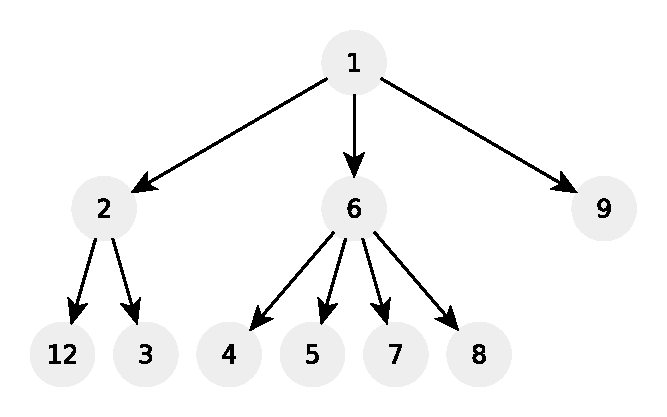
\includegraphics[scale=1.0]{sources/node_from_the_end/images/example1}
	\caption{Removal of the \nth{2} to last element in a singly linked list of length $4$.}
\end{figure}

\begin{figure}
	\label{fig:node_from_the_end:example2}
	\centering
	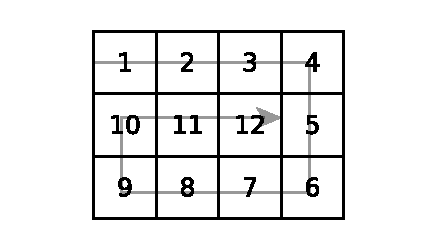
\includegraphics[scale=1.0]{sources/node_from_the_end/images/example2}
	\caption{Removal of the \nth{4} to last element in a singly linked list of legth $4$. The head pointer needs to be updated.}
\end{figure}


\section{Clarification Questions}

\begin{QandA}
	\item 
	\begin{answered}
		\textit{}
	\end{answered}
	
\end{QandA}

\section{Discussion}
\label{node_from_the_end:sec:discussion}


\subsection{Brute-force}
\label{node_from_the_end:sec:bruteforce}

\lstinputlisting[language=c++, caption={Sample Caption},label=list:node_from_the_end]{sources/node_from_the_end/node_from_the_end_solution1.cpp}



\subsection{Common Variation }
\subsubsection{List midpoint}
\label{node_from_the_end:sec:list_midpoint}